\section{Introduction}
\label{sec:intro}

In this section, we provide reasons to learn about the Gauss-Bonnet theorem. We then consider a special case of the theorem for simple polygons and we use this special case to prove Pick's theorem.

\subsection{A Great Theorem}
The Gauss-Bonnet theorem relates the curvature, a local property, of a surface
to the Euler characteristic, a global property. If we travel over a surface and compute the curvature
at each point we are able to combine our computations to learn about the topology of the surface
as a whole. Conversely, if we know the topology of a surface we are able to 
guarantee the existence of a point on the surface with positive curvature. 
The goal of this work is to demonstrate that both of the directions described above are useful.


In symbols, a version of the Gauss-Bonnet theorem can be expressed as

\begin{equation}\label{eqn:g-b-noboundary}
		\int_MK dA =2\pi \chi(M)
\end{equation}
where $M$ is a smooth surface in $\RR^3$ without boundary, $K$ is Gaussian curvature
and $\chi(M)$ is the Euler characteristic of $M$.


The Gauss-Bonnet theorem is a hub between seemingly disparate ideas, see \figref{bridge}. 

\begin{figure}[htb]
\centering
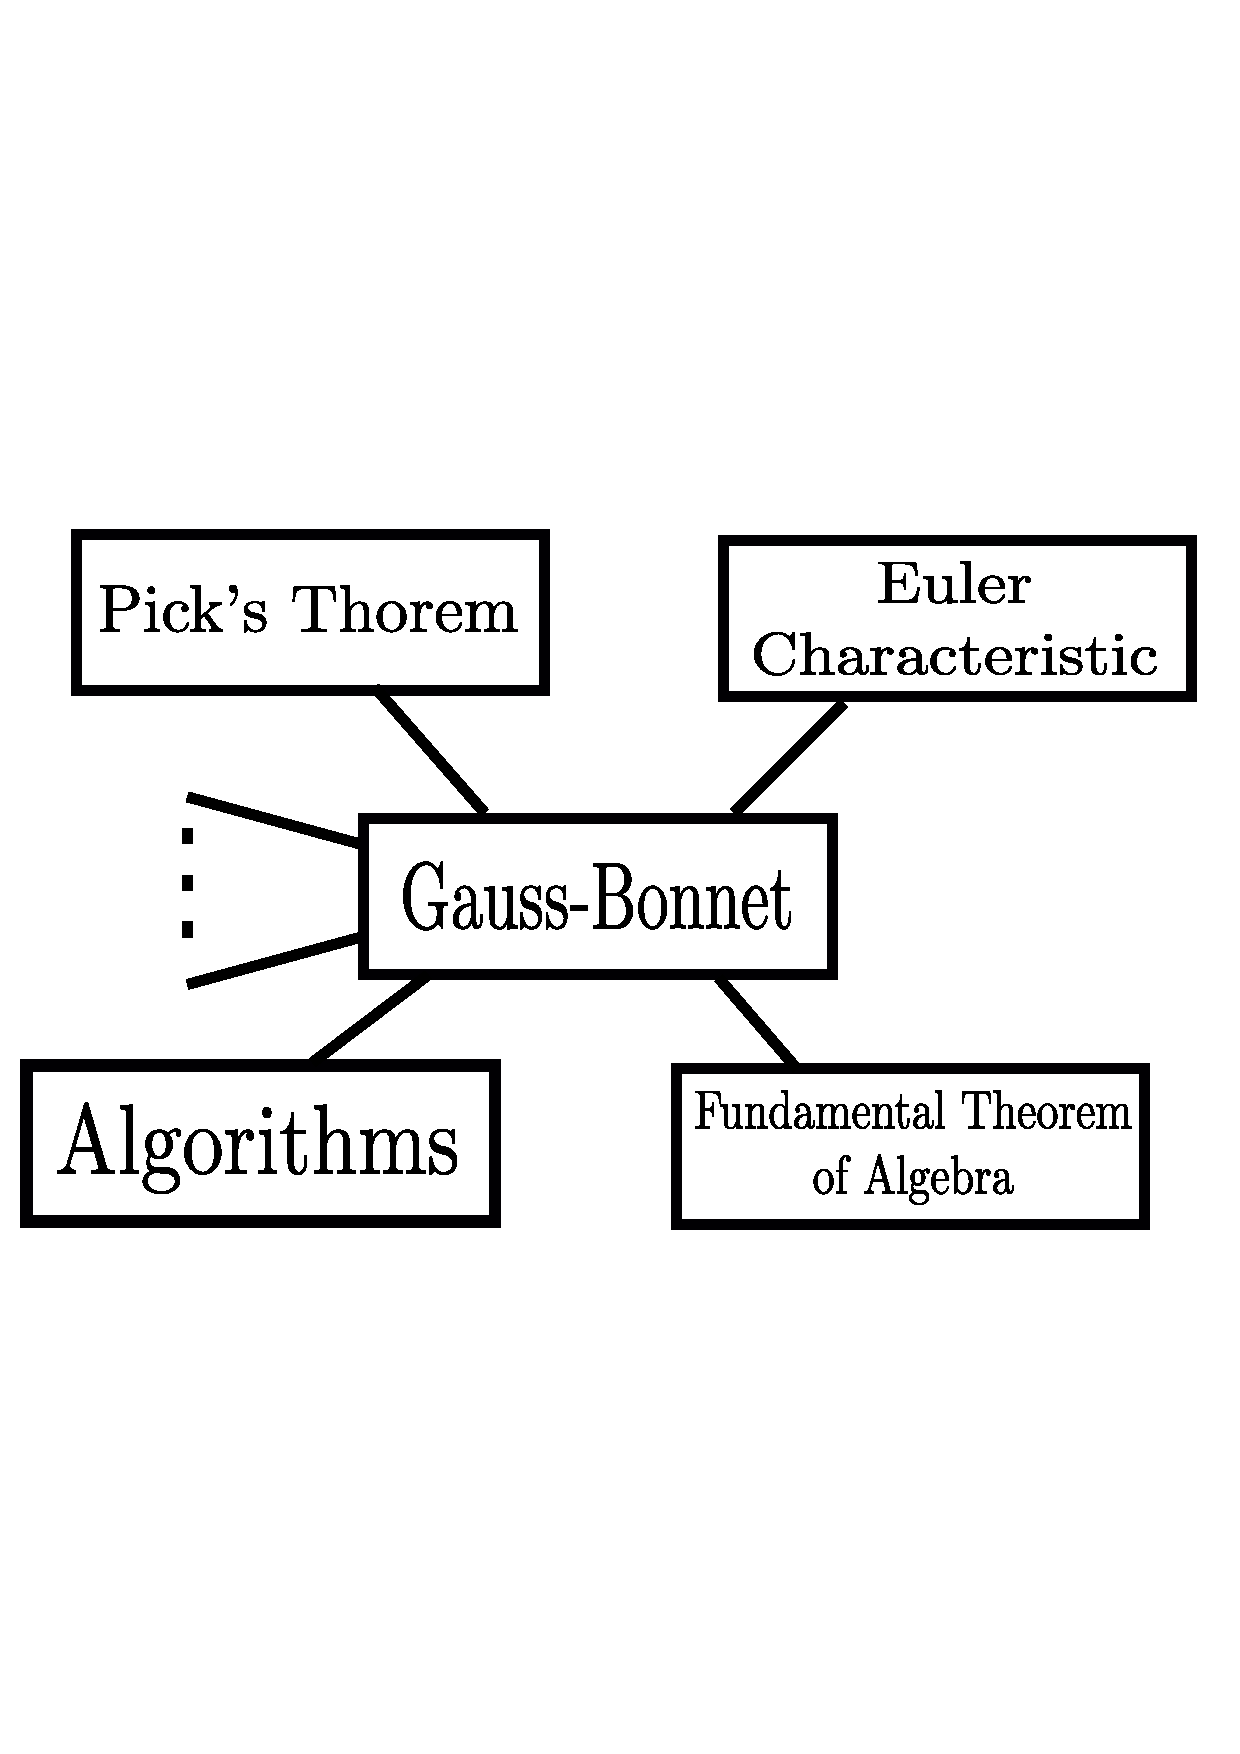
\includegraphics[width=.3\textwidth]{curvature/bridge}
\caption{The Gauss-Bonnet theorem is a star.}
\label{fig:bridge}
\end{figure}

What separates a great theorem form a mediocre theorem?
In \cite{jm08}, Matou\v{s}ek says that a theorem is a great theorem if there are
\begin{enumerate}[(1)]
\item several different equivalent versions,
\item many different proofs,
\item a host of extensions and generalizations, and
\item numerous interesting applications.
\end{enumerate}

By this criteria, the Gauss-Bonnet theorem is a great theorem.
For (1), six different versions of the theorem are discussed
in \cite{wu_historical_2008}. 
In addition to the version for smooth surfaces given in \eqnref{g-b-noboundary},
we highlight several discrete versions for triangulated surfaces. 
 
 
 
As for (2), several fundamentally different proofs exist.  
One common approach is to first prove the theorem for simply connected domains
with boundary, then triangulate a surface and add up the contribution from each triangle.
However, this proof seems to lack a geometric intuition that other proofs provide. \cite{wu_historical_2008},
A second commonly seen proof is to use Stokes theorem  \cite{doc76,pressley_elementary_2010}.
Many other proofs exist \cite{guillemin_differential_2010,levi-bicycle,grinfeld_introduction_2013}.


For (3), the theorem has been generalized in the following ways.
The two notable examples are the Chern-Gauss-Bonnet theorem\cite{chern_simple_1944} and
the Atiyah–Singer index theorem is an example  \cite{atiyah_index_1963}.
A generalization to higher dimensions \cite{guillemin_differential_2010}.
The discrete versions of the theorem discussed here can be thought of as extensions
to more computationally friendly objects.



As for (4), applications, 
seven are given in \cite{doc76}.
For applications to physics see \cite{tirado-physics-apps,gibbons_applications_2008}.
This work provides examples related to the algorithms and combinatorics but we include
others.
I hope that the number of applications continues to grow,
please share any that you feel
ought to be included\footnote{\text{mccoy2ba@jmu.edu}}.

Thus, by Matou\v{s}ek standard, the Gauss-Bonnet theorem is a great theorem.
We highlight classic applications of the theorem as well as more recent
applications that illustrate that topological methods in combinatorics is an active
area of research.

Historically,  Gauss proved the special case of a geodesic triangle\cite{dombrowski-79,gauss_disquisitiones_1827}.  
The version given in \eqnref{g-b-noboundary} is due to Pierre Bonnet
and Jacques Binet \cite{bonnet1848memoire}. A case can be made that the theorem
ought to be called the Bauss-Binet-Bonnet Theorem
\cite{wu_historical_2008}.

\subsection{Simple Polygons}
\label{sec:warm-up}

Some of us may remember the following special case
of the Gauss-Bonnet theorem from geometry in secondary school.
Consider a simple polygon $P$, an example is shown in \figref{polygon}.

 \begin{figure}[htb]
         \centering
          \begin{subfigure}[b]{0.30\textwidth}
      		   \includegraphics[width=\textwidth]{background/blank-polygon}
    		    \caption{A simple polygon.}
 		 \label{fig:polygon}
	 \end{subfigure}
	 \hspace{.5cm}
	 \begin{subfigure}[b]{0.25\textwidth}
       		  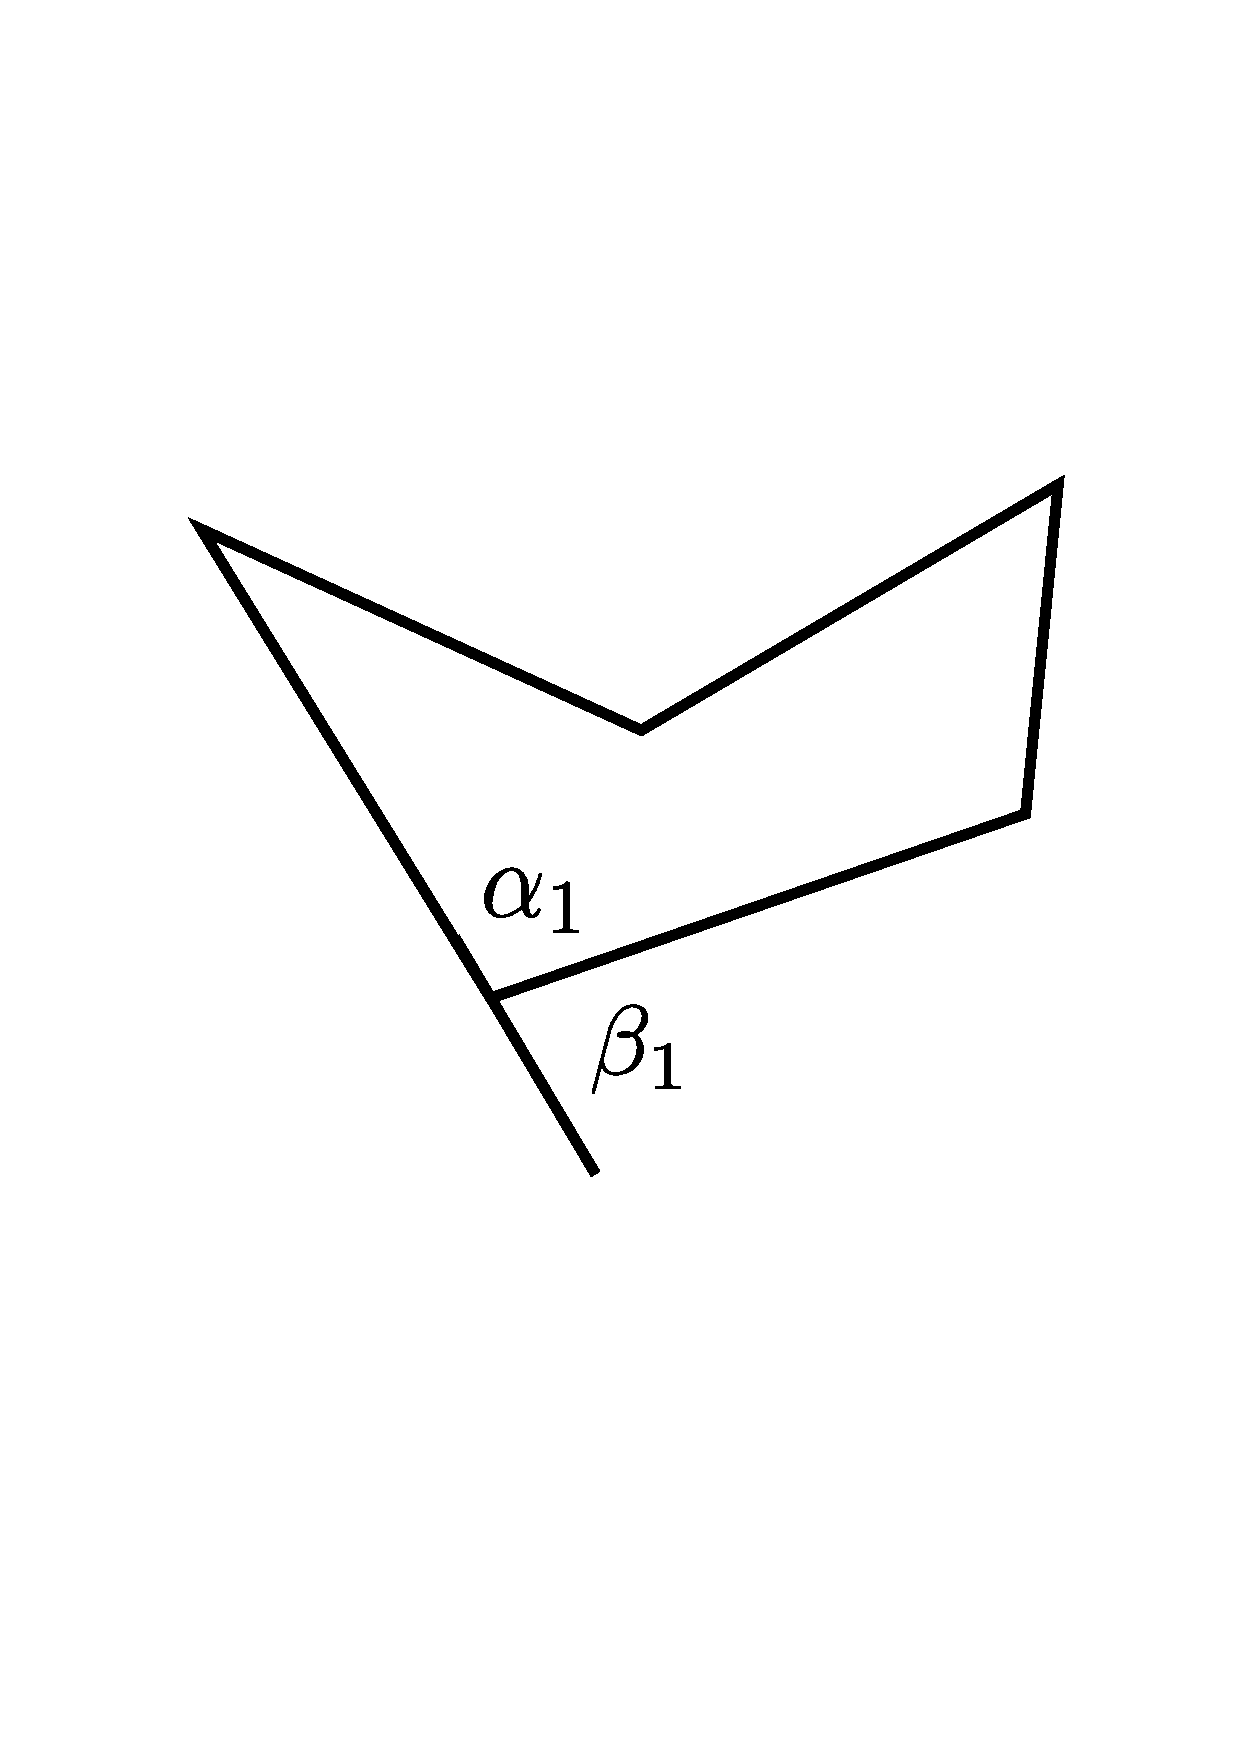
\includegraphics[width=\textwidth]{background/interior-exterior}
     		    \caption{Angles}
 		 \label{fig:interior-exterior}
       \end{subfigure}
        \hspace{.5cm}
     \begin{subfigure}[b]{0.27\textwidth}
       		  \includegraphics[width=\textwidth]{background/exterior-angles-polygon}
       		  \caption{Exterior angles.}
       		   \label{fig:exterior-angles}
         \end{subfigure}
		\caption{(\subref{fig:polygon}) A simple polygon $P.$
		(\subref{fig:interior-exterior}) The interior and exterior angles formed at a vertex.
 		 (\subref{fig:exterior-angles}) The sum of the exterior angles of a simple
		polygon is $2\pi$. Here
		$\beta_1+\beta_2+\beta_3+\beta_4+\beta_5=2\pi$ note that $\beta_4$ is negative.
 		\label{fig:simple-polygon}}
 \end{figure}

If we extend one side of $P$ at a vertex two complementary angles appear.
An example is shown in \figref{interior-exterior}.
The angle inside $P$ is the \EMPH{interior} angle and the complement 
is the  \EMPH{exterior angle}. 
Vertices with interior angle greater than $\pi$ are called \EMPH{reflex},
an example is shown at $\beta_4$ in \figref{exterior-angles}.
If we imagine walking counterclockwise around $P$, at reflex angles we turn right.
Note that at reflex angles, the exterior angle inside of $P$, thus we define
these exterior angles to be negative. 


We now state a simple version of the Gauss-Bonnet theorem \cite{gottlieb_all_1996,polya_elementary_1954},

\begin{theorem}[Gauss-Bonnet for Simple Polygons in the Plane]\label{thm:simple-bonnet}
Let $P$ be a simple polygon in the plane with $n$  vertices,
interior angles $\{\alpha_1,\alpha_2,\ldots,\alpha_n\}$
and exterior angles $\{\beta_1,\beta_2,\ldots,\beta_n\}$ then
\begin{equation}\label{eqn:exterior-sum}
		\sum_{i=1}^n\beta_i=2\pi
\end{equation}

and 
\begin{equation}\label{eqn:interior-sum}
		\sum_{i=1}^n\alpha_i=\pi(n-2).
\end{equation}

\end{theorem}


\begin{proof}

	We traverse a polygon and rotate $\beta_i$ at each vertex
	when we get back to where we started we will have preformed 
	one complete revolution so $\sum_{i=1}^n\beta_i=2\pi.$
	The exterior angles are complementary to the interior angles
	so for each $i$ we have $\beta_i=\pi-\alpha_i$  and, using \eqnref{exterior-sum},
	  we have
	$\sum_{i=1}^n(\pi-\alpha_i)=n\pi -\sum_{i=1}^n\alpha_i=2\pi$. 
	Solving for $\sum_{i=1}^n\alpha_i$ gives the second part of the theorem.

\end{proof}
No matter how we position the vertices of our polygon,
if the boundary of the polygon stays closed and simple,
the sum the exterior angles will be $2\pi$.
Even this simple version of the Gauss-Bonnet theorem has powerful
consequences, as we now see in our first application, a proof of Pick's Theorem.



\subsection{Pick's Theorem}
\label{sec:pick}

Pick's Theorem gives a formula for the area of a polygon
in the plane with vertices on the lattice $\ZZ^2$ \cite{og-pick}.
We give a proof originally due to Blatter \cite{blatter_another_1997}
and restated by Tabachnikov  \cite{tabachnikov_proofs_2014}.

\begin{theorem}[Pick's Theorem]\label{thm:pick}
Let $P$ be a simple polygon in the plane with vertices on the lattice $\ZZ^2$,
let $I$ be the number of lattice points inside of $P$, let $B$ be the number
of lattice points on the boundary of $P$ and let $A$ denote the area of $P$.
Then, 
$$A=I+\frac{B}{2}-1.$$
\end{theorem}
See \figref{picks} for an example.

 \begin{figure}[htb]
         \centering
         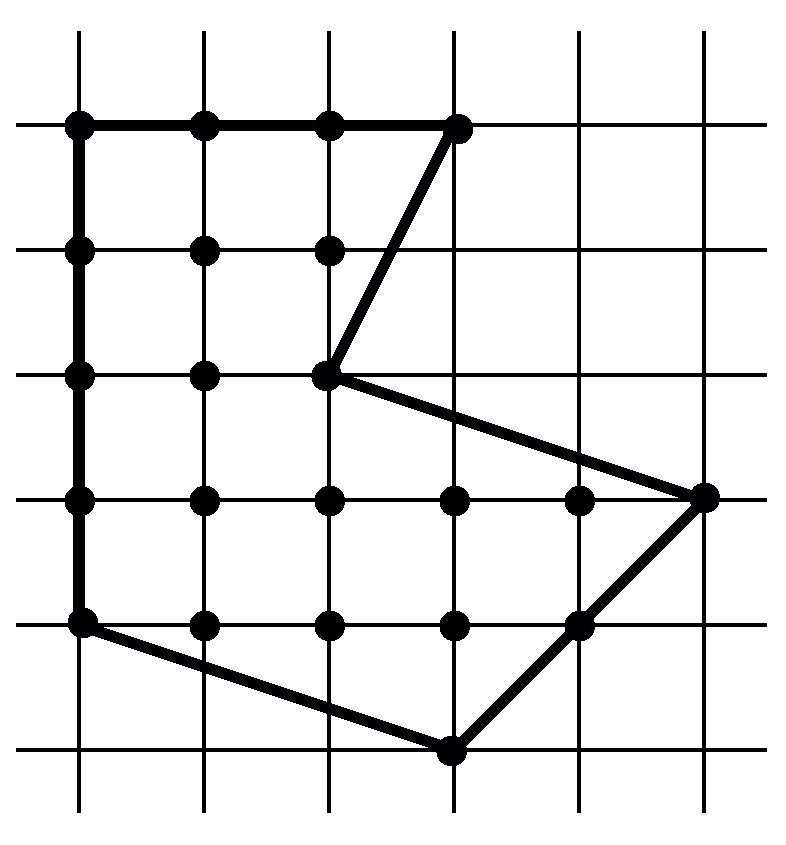
\includegraphics[width=5cm]{pick}
	\caption{A polygon with vertices on the lattice. 
	There are 10 interior vertices and 12 vertices on the boundary.
	By Pick's theorem the area of the polygon is $10+\frac{12}{2}-1=15.$
	\label{fig:picks}}
 \end{figure}
 
\begin{proof}
	Consider a unit volume ice cube at each lattice point in the plane and let the ice melt.
	The water will evenly cover the plane with the amount of water inside the polygon 
	equal to its area.
	
	An edge of the polygon connects two lattice points,
	for each ice cube the contributes flow across the edge in one direction there is a symmetric
	point that contributes an equal amount of flow in the opposite direction. Thus, 
	the amount of water that flows
	into to polygon across this edge equals that amount of water that flows out of the polygon
	across this edge by symmetry.
	So, the total flow across each edge is zero and
	the amount of water inside the polygon can be considered to come from ice cubes interior to the polygon and the cubes on the vertices
	of the polygon.
	
	Each interior lattice point contributes one unit of water. 
	Each lattice point on an edge, half of the water flows into the polygon and
	half flows outside of the polygon.
	Let $\alpha_i$ denote the interior angles at each vertex.
	Each vertex contributes $\frac{\alpha_i}{2\pi}$ units of water to the area.
	By the Gauss-Bonnet theorem, \thmref{simple-bonnet}, the sum of the interior
	angles is $\pi(n-2)$. Thus, the vertex points contribute a total of 
	$$\frac{\pi(n-2)}{2\pi}=\frac{n}{2}-1.$$
	The number of boundary points $B$ is $n$ plus the number of lattice points interior to an edge
	and we have
	$$A=I+\frac{B}{2}-1.$$
\end{proof}


\noindent \textbf{Exercises}


\begin{enumerate}
	\item Use Pick's theorem to prove that you cannot draw an equilateral triangle by with its vertices
	at grid points.
	
	\item Fix an integer $N$, consider all positive rational number $\frac{a}{b}$ where
	$b\leq N$. Place them in increasing order. This is a called the \EMPH{Farey sequence}.
	For example, when $N=3$, we have
	$$\frac{0}{1}<\frac{1}{3}<\frac{1}{2}<\frac{2}{3}<\frac{1}{1}<\frac{4}{3}<\ldots.$$
	For two consecutive terms in a Farey sequence $\frac{a}{b}<\frac{c}{d}$ in lowest terms,
	prove $bc-ad=1.$
	
\end{enumerate}

\pagebreak
